% Created by tikzDevice version 0.12.6 on 2026-08-03 04:28:21
% !TEX encoding = UTF-8 Unicode
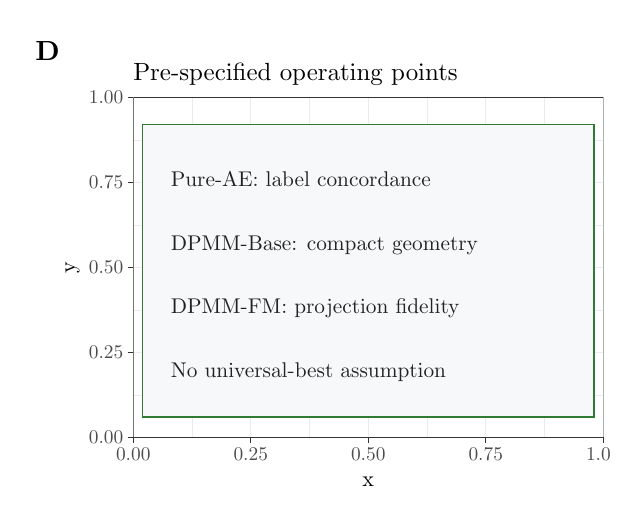
\begin{tikzpicture}[x=1pt,y=1pt]
\definecolor{fillColor}{RGB}{255,255,255}
\path[use as bounding box,fill=fillColor,fill opacity=0.00] (0,0) rectangle (210.78,171.36);
\begin{scope}
\path[clip] (  0.79,  1.87) rectangle (209.99,169.49);
\definecolor{drawColor}{RGB}{255,255,255}
\definecolor{fillColor}{RGB}{255,255,255}

\path[draw=drawColor,line width= 0.4pt,line join=round,line cap=round,fill=fillColor] (  0.79,  1.87) rectangle (209.99,169.49);
\end{scope}
\begin{scope}
\path[clip] ( 38.15, 23.34) rectangle (207.99,146.20);
\definecolor{fillColor}{RGB}{255,255,255}

\path[fill=fillColor] ( 38.15, 23.34) rectangle (207.99,146.20);
\definecolor{drawColor}{gray}{0.92}

\path[draw=drawColor,line width= 0.2pt,line join=round] ( 38.15, 38.69) --
	(207.99, 38.69);

\path[draw=drawColor,line width= 0.2pt,line join=round] ( 38.15, 69.41) --
	(207.99, 69.41);

\path[draw=drawColor,line width= 0.2pt,line join=round] ( 38.15,100.12) --
	(207.99,100.12);

\path[draw=drawColor,line width= 0.2pt,line join=round] ( 38.15,130.84) --
	(207.99,130.84);

\path[draw=drawColor,line width= 0.2pt,line join=round] ( 59.38, 23.34) --
	( 59.38,146.20);

\path[draw=drawColor,line width= 0.2pt,line join=round] (101.84, 23.34) --
	(101.84,146.20);

\path[draw=drawColor,line width= 0.2pt,line join=round] (144.30, 23.34) --
	(144.30,146.20);

\path[draw=drawColor,line width= 0.2pt,line join=round] (186.76, 23.34) --
	(186.76,146.20);

\path[draw=drawColor,line width= 0.4pt,line join=round] ( 38.15, 23.34) --
	(207.99, 23.34);

\path[draw=drawColor,line width= 0.4pt,line join=round] ( 38.15, 54.05) --
	(207.99, 54.05);

\path[draw=drawColor,line width= 0.4pt,line join=round] ( 38.15, 84.77) --
	(207.99, 84.77);

\path[draw=drawColor,line width= 0.4pt,line join=round] ( 38.15,115.48) --
	(207.99,115.48);

\path[draw=drawColor,line width= 0.4pt,line join=round] ( 38.15,146.20) --
	(207.99,146.20);

\path[draw=drawColor,line width= 0.4pt,line join=round] ( 38.15, 23.34) --
	( 38.15,146.20);

\path[draw=drawColor,line width= 0.4pt,line join=round] ( 80.61, 23.34) --
	( 80.61,146.20);

\path[draw=drawColor,line width= 0.4pt,line join=round] (123.07, 23.34) --
	(123.07,146.20);

\path[draw=drawColor,line width= 0.4pt,line join=round] (165.53, 23.34) --
	(165.53,146.20);

\path[draw=drawColor,line width= 0.4pt,line join=round] (207.99, 23.34) --
	(207.99,146.20);
\definecolor{drawColor}{RGB}{46,125,50}
\definecolor{fillColor}{RGB}{247,248,250}

\path[draw=drawColor,line width= 0.5pt,fill=fillColor] ( 41.55, 30.71) rectangle (204.59,136.37);
\definecolor{drawColor}{RGB}{34,34,34}

\node[text=drawColor,anchor=base west,inner sep=0pt, outer sep=0pt, scale=  0.77] at ( 51.74,113.88) {Pure-AE: label concordance};

\node[text=drawColor,anchor=base west,inner sep=0pt, outer sep=0pt, scale=  0.77] at ( 51.74, 90.94) {DPMM-Base: compact geometry};

\node[text=drawColor,anchor=base west,inner sep=0pt, outer sep=0pt, scale=  0.77] at ( 51.74, 68.01) {DPMM-FM: projection fidelity};

\node[text=drawColor,anchor=base west,inner sep=0pt, outer sep=0pt, scale=  0.77] at ( 51.74, 45.08) {No universal-best assumption};
\definecolor{drawColor}{gray}{0.20}

\path[draw=drawColor,line width= 0.4pt,line join=round,line cap=round] ( 38.15, 23.34) rectangle (207.99,146.20);
\end{scope}
\begin{scope}
\path[clip] (  0.00,  0.00) rectangle (210.78,171.36);
\definecolor{drawColor}{gray}{0.30}

\node[text=drawColor,anchor=base east,inner sep=0pt, outer sep=0pt, scale=  0.70] at ( 34.55, 20.93) {0.00};

\node[text=drawColor,anchor=base east,inner sep=0pt, outer sep=0pt, scale=  0.70] at ( 34.55, 51.64) {0.25};

\node[text=drawColor,anchor=base east,inner sep=0pt, outer sep=0pt, scale=  0.70] at ( 34.55, 82.36) {0.50};

\node[text=drawColor,anchor=base east,inner sep=0pt, outer sep=0pt, scale=  0.70] at ( 34.55,113.07) {0.75};

\node[text=drawColor,anchor=base east,inner sep=0pt, outer sep=0pt, scale=  0.70] at ( 34.55,143.79) {1.00};
\end{scope}
\begin{scope}
\path[clip] (  0.00,  0.00) rectangle (210.78,171.36);
\definecolor{drawColor}{gray}{0.20}

\path[draw=drawColor,line width= 0.4pt,line join=round] ( 36.15, 23.34) --
	( 38.15, 23.34);

\path[draw=drawColor,line width= 0.4pt,line join=round] ( 36.15, 54.05) --
	( 38.15, 54.05);

\path[draw=drawColor,line width= 0.4pt,line join=round] ( 36.15, 84.77) --
	( 38.15, 84.77);

\path[draw=drawColor,line width= 0.4pt,line join=round] ( 36.15,115.48) --
	( 38.15,115.48);

\path[draw=drawColor,line width= 0.4pt,line join=round] ( 36.15,146.20) --
	( 38.15,146.20);
\end{scope}
\begin{scope}
\path[clip] (  0.00,  0.00) rectangle (210.78,171.36);
\definecolor{drawColor}{gray}{0.20}

\path[draw=drawColor,line width= 0.4pt,line join=round] ( 38.15, 21.34) --
	( 38.15, 23.34);

\path[draw=drawColor,line width= 0.4pt,line join=round] ( 80.61, 21.34) --
	( 80.61, 23.34);

\path[draw=drawColor,line width= 0.4pt,line join=round] (123.07, 21.34) --
	(123.07, 23.34);

\path[draw=drawColor,line width= 0.4pt,line join=round] (165.53, 21.34) --
	(165.53, 23.34);

\path[draw=drawColor,line width= 0.4pt,line join=round] (207.99, 21.34) --
	(207.99, 23.34);
\end{scope}
\begin{scope}
\path[clip] (  0.00,  0.00) rectangle (210.78,171.36);
\definecolor{drawColor}{gray}{0.30}

\node[text=drawColor,anchor=base,inner sep=0pt, outer sep=0pt, scale=  0.70] at ( 38.15, 14.92) {0.00};

\node[text=drawColor,anchor=base,inner sep=0pt, outer sep=0pt, scale=  0.70] at ( 80.61, 14.92) {0.25};

\node[text=drawColor,anchor=base,inner sep=0pt, outer sep=0pt, scale=  0.70] at (123.07, 14.92) {0.50};

\node[text=drawColor,anchor=base,inner sep=0pt, outer sep=0pt, scale=  0.70] at (165.53, 14.92) {0.75};

\node[text=drawColor,anchor=base,inner sep=0pt, outer sep=0pt, scale=  0.70] at (207.99, 14.92) {1.00};
\end{scope}
\begin{scope}
\path[clip] (  0.00,  0.00) rectangle (210.78,171.36);
\definecolor{drawColor}{RGB}{0,0,0}

\node[text=drawColor,anchor=base,inner sep=0pt, outer sep=0pt, scale=  0.80] at (123.07,  5.64) {x};
\end{scope}
\begin{scope}
\path[clip] (  0.00,  0.00) rectangle (210.78,171.36);
\definecolor{drawColor}{RGB}{0,0,0}

\node[text=drawColor,rotate= 90.00,anchor=base,inner sep=0pt, outer sep=0pt, scale=  0.80] at ( 17.12, 84.77) {y};
\end{scope}
\begin{scope}
\path[clip] (  0.00,  0.00) rectangle (210.78,171.36);
\definecolor{drawColor}{RGB}{0,0,0}

\node[text=drawColor,anchor=base west,inner sep=0pt, outer sep=0pt, scale=  0.90] at ( 38.15,152.18) {Pre-specified operating points};
\end{scope}
\begin{scope}
\path[clip] (  0.00,  0.00) rectangle (210.78,171.36);
\definecolor{drawColor}{RGB}{0,0,0}

\node[text=drawColor,anchor=base,inner sep=0pt, outer sep=0pt, scale=  1.00] at (  7.20,159.49) {\bfseries D};
\end{scope}
\end{tikzpicture}
